\documentclass[tikz,border=12pt]{standalone}
\usepackage{amsmath}
\usepackage{amssymb}
\usepackage{tikz}
\usetikzlibrary{arrows.meta}

\definecolor{ink}{HTML}{0F172A}
\definecolor{linegray}{HTML}{64748B}
\definecolor{visible}{HTML}{E2E8F0}
\definecolor{masked}{HTML}{F8FAFC}
\definecolor{maskedge}{HTML}{94A3B8}

\begin{document}
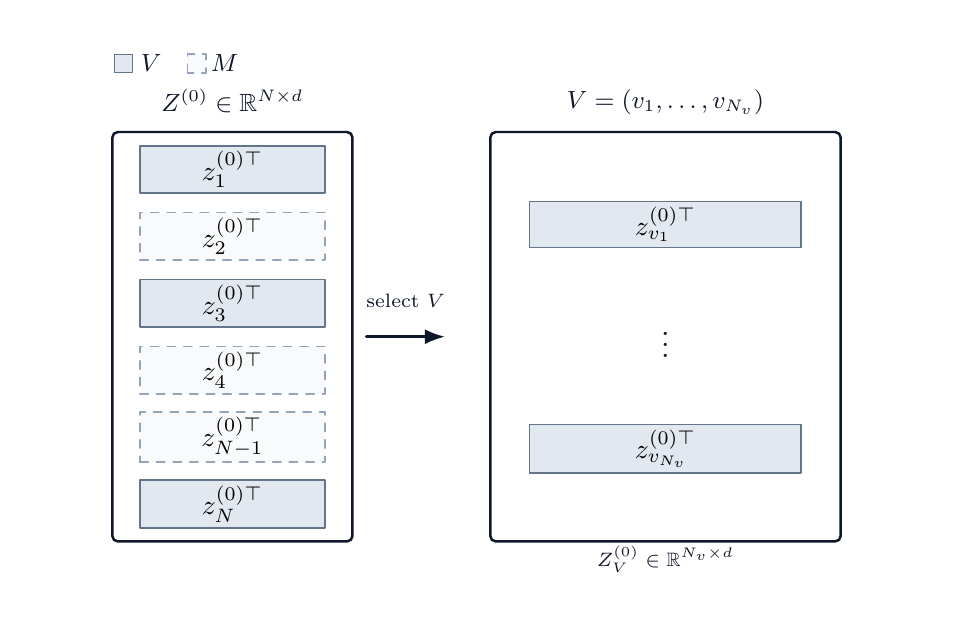
\begin{tikzpicture}[
  font=\sffamily,
  >=Latex,
  line cap=round,
  line join=round,
  token/.style={
    draw=linegray,
    line width=0.6pt,
    minimum width=2.35cm,
    minimum height=0.52cm,
    inner sep=2pt,
    align=center
  },
  masked token/.style={
    token,
    draw=maskedge,
    dashed,
    fill=masked
  }
]
  \fill[white] (-0.55,-0.8) rectangle (11.1,6.55);

  % The same row-wise token matrix introduced in Figure 4.
  \node[ink, font=\small] at (2.05,5.62)
    {$Z^{(0)} \in \mathbb{R}^{N\times d}$};
  \node[draw=ink, line width=0.9pt, rounded corners=2pt,
    minimum width=3.05cm, minimum height=5.2cm, fill=white,
    inner sep=0pt] at (2.05,2.625) {};
  \node[token, fill=visible] at (2.05,4.75)
    {$z_1^{(0)\top}$};
  \node[masked token] at (2.05,3.9)
    {$z_2^{(0)\top}$};
  \node[token, fill=visible] at (2.05,3.05)
    {$z_3^{(0)\top}$};
  \node[masked token] at (2.05,2.2)
    {$z_4^{(0)\top}$};
  \node[masked token] at (2.05,1.35)
    {$z_{N-1}^{(0)\top}$};
  \node[token, fill=visible] at (2.05,0.5) {$z_N^{(0)\top}$};

  % The visible/masked legend applies to rows in the matrix.
  \fill[visible] (0.55,5.98) rectangle (0.78,6.21);
  \draw[linegray, line width=0.45pt] (0.55,5.98) rectangle (0.78,6.21);
  \node[ink, font=\small] at (1.02,6.1) {$V$};
  \fill[masked] (1.48,5.98) rectangle (1.71,6.21);
  \draw[maskedge, dashed, line width=0.7pt]
    (1.48,5.98) rectangle (1.71,6.21);
  \node[ink, font=\small] at (1.95,6.1) {$M$};

  \draw[ink, ->, line width=0.95pt] (3.75,2.625) -- (4.75,2.625);
  \node[ink, font=\scriptsize, fill=white, inner sep=1pt, anchor=south]
    at (4.25,2.95)
    {$\text{select }V$};

  % Only the visible rows are retained in the encoder input.
  \node[draw=ink, line width=0.9pt, rounded corners=2pt,
    minimum width=4.45cm, minimum height=5.2cm, fill=white,
    inner sep=0pt] at (7.55,2.625) {};
  \node[ink, font=\small, fill=white, inner sep=1pt] at (7.55,5.6)
    {$V=(v_1,\ldots,v_{N_v})$};
  \node[token, fill=visible, minimum width=3.45cm] at (7.55,4.05)
    {$z_{v_1}^{(0)\top}$};
  \node[ink, font=\large] at (7.55,2.625) {$\vdots$};
  \node[token, fill=visible, minimum width=3.45cm] at (7.55,1.2)
    {$z_{v_{N_v}}^{(0)\top}$};
  \node[ink, font=\scriptsize] at (7.55,-0.2)
    {$Z_V^{(0)}\in\mathbb{R}^{N_v\times d}$};
\end{tikzpicture}
\end{document}
